\section{Descrizione del prodotto}

\subsection{Obiettivi del prodotto}
Il progetto ha come obiettivo la realizzazione di una piattaforma che consenta di 
gestire un assistente virtuale per la conoscenza e la descrizione di bevande, 
sfruttando un’infrastruttura basata su modelli linguistici di grandi dimensioni. 
La piattaforma dovrà supportare le richieste degli utenti in modo rapido, 
preciso e sempre disponibile, eliminando la necessità di uno specialista fisico. 
Essa permetterà la consultazione di informazioni dettagliate su prodotti come caratteristiche, 
formati disponibili e suggerimenti d’uso, adattandosi alle esigenze specifiche 
dei clienti e garantendo un’interazione fluida in linguaggio naturale. 
L’assistente virtuale sarà progettato per integrarsi con database aziendali, 
sfruttando le informazioni esistenti per rispondere alle domande in modo 
contestualizzato e accurato.

\subsection{Architettura del prodotto}
I componenti del prodotto sono:
\begin{itemize}
    \item \href{https://code7crusaders.github.io/docs/RTB/documentazione_interna/glossario.html#database-relazionale}{\textbf{Database Relazionale}\textsuperscript{G}}:  
    Questo componente memorizza i dati strutturati dell’azienda, come descrizioni di prodotti, ingredienti, specifiche tecniche e altro. È il punto di partenza per acquisire informazioni utili che saranno processate e utilizzate dal sistema. Supporta query SQL per consentire l'accesso rapido e organizzato ai dati.
    
    \item \href{https://code7crusaders.github.io/docs/RTB/documentazione_interna/glossario.html#embedding}{\textbf{Embedding\textsuperscript{G}} Model}:  
    L’Embedding Model è un modello pre-addestrato in grado di trasformare il testo in rappresentazioni numeriche preservando il significato semantico. Viene utilizzato sia per i dati aziendali durante l’addestramento che per le domande poste dagli utenti. Gli embedding risultanti permettono confronti efficienti nel \href{https://code7crusaders.github.io/docs/RTB/documentazione_interna/glossario.html#database-vettoriale}{database vettoriale\textsuperscript{G}}.
    
    \item \href{https://code7crusaders.github.io/docs/RTB/documentazione_interna/glossario.html#database-vettoriale}{\textbf{Database Vettoriale}\textsuperscript{G}}:  
    Questo componente archivia i vettori generati dall’\href{https://code7crusaders.github.io/docs/RTB/documentazione_interna/glossario.html#embedding}{Embedding\textsuperscript{G}} Model. Utilizza indicizzazione ottimizzata per operazioni di \href{https://code7crusaders.github.io/docs/RTB/documentazione_interna/glossario.html#nearest-neighbor-search-nns}{\textit{nearest neighbor search}\textsuperscript{G}}, permettendo di trovare rapidamente i vettori più simili a una query. È il cuore della fase di recupero delle informazioni nel sistema.
    
    \item \href{https://code7crusaders.github.io/docs/RTB/documentazione_interna/glossario.html#llm-large-language-model}{\textbf{LLM}\textsuperscript{G}}:  
    Il Large Language Model riceve in input il contesto fornito dal \href{https://code7crusaders.github.io/docs/RTB/documentazione_interna/glossario.html#database-vettoriale}{database vettoriale\textsuperscript{G}} e la domanda dell’utente. Grazie alla sua capacità generativa, l'\href{https://code7crusaders.github.io/docs/RTB/documentazione_interna/glossario.html#llm-large-language-model}{LLM\textsuperscript{G}} riceve in input il contesto fornito dal database vettoriale e la domanda dell’utente. Grazie alla sua capacità generativa, il LLM elabora risposte dettagliate e accurate, combinando i dati presenti con la comprensione del linguaggio naturale.
    
    \item \textbf{Web App}:  
    La Web App è l’interfaccia attraverso la quale gli utenti interagiscono con il sistema. Fornisce un’esperienza semplice e intuitiva per inserire domande e visualizzare risposte. Comunica con il backend tramite \href{https://code7crusaders.github.io/docs/RTB/documentazione_interna/glossario.html#api-rest-representational-state-transfer}{API REST\textsuperscript{G}} per garantire un'interazione rapida e scalabile.
\end{itemize}

\subsection{Implementazione scelta: LLM e strumenti}
\subsubsection{Scelta dell'LLM}
Dopo un'attenta analisi comparativa tra i modelli di Huggingface (BLOOM e varianti) e OpenAI (GPT-4o e GPT-4omini) nel file di \textbf{analisi modelli.pdf}, si è optato per l'utilizzo di GPT-4omini di OpenAI. La scelta è motivata dai seguenti fattori:
\begin{itemize}
    \item \textbf{Prestazioni}: GPT-4omini offre risultati superiori rispetto ai modelli open-source in termini di accuratezza e capacità di generazione del linguaggio, come evidenziato dai \href{https://code7crusaders.github.io/docs/RTB/documentazione_interna/glossario.html#benchmark}{benchmark\textsuperscript{G}} \textbf{analisi modelli}.
    \item \href{https://code7crusaders.github.io/docs/RTB/documentazione_interna/glossario.html#scalabilità}{\textbf{Scalabilità}\textsuperscript{G}}: Le API di OpenAI garantiscono un'infrastruttura cloud scalabile, eliminando i costi e la complessità legati alla gestione locale di modelli di grandi dimensioni.
    \item \textbf{Costi ottimizzati}: Il costo basato sui \href{https://code7crusaders.github.io/docs/RTB/documentazione_interna/glossario.html#token}{token\textsuperscript{G}} elaborati permette un utilizzo flessibile e sostenibile, adattandosi alle esigenze di carico variabile del sistema.
\end{itemize}

\subsubsection{Pipeline di Implementazione}
L'implementazione sfrutta un'architettura RAG (Retrieval-Augmented Generation), integrando i seguenti componenti:
\begin{enumerate}
    \item Generazione degli Embedding: Le informazioni aziendali (es. cataloghi di prodotti) vengono preprocessate e trasformate in vettori numerici tramite \href{https://code7crusaders.github.io/docs/RTB/documentazione_interna/glossario.html#bert-bidirectional-encoder-representations-from-transformers}{BERT\textsuperscript{G}}\href{https://code7crusaders.github.io/docs/RTB/documentazione_interna/glossario.html#embedding}{Embedding\textsuperscript{G}}: Le informazioni aziendali (es. cataloghi di prodotti) vengono preprocessate e trasformate in vettori numerici tramite BERT di Huggingface.
    \item Archiviazione degli \href{https://code7crusaders.github.io/docs/RTB/documentazione_interna/glossario.html#embedding}{Embedding\textsuperscript{G}}: I vettori generati vengono memorizzati e indicizzati utilizzando \href{https://code7crusaders.github.io/docs/RTB/documentazione_interna/glossario.html#faiss}{FAISS\textsuperscript{G}}, che consente un recupero efficiente dei dati rilevanti.
    \item Integrazione con LLM: Le domande degli utenti, trasformate in embedding, vengono confrontate con il \href{https://code7crusaders.github.io/docs/RTB/documentazione_interna/glossario.html#database-vettoriale}{database vettoriale\textsuperscript{G}}. Il contesto recuperato viene passato a GPT-4omini per generare risposte accurate e personalizzate.
    \item Web App e \href{https://code7crusaders.github.io/docs/RTB/documentazione_interna/glossario.html#api-rest-representational-state-transfer}{API REST\textsuperscript{G}}: La comunicazione tra frontend (React) e backend avviene tramite \href{https://code7crusaders.github.io/docs/RTB/documentazione_interna/glossario.html#api-rest-representational-state-transfer}{API REST\textsuperscript{G}}, garantendo tempi di risposta rapidi.
\end{enumerate}

\subsubsection{Motivazione degli Strumenti Scelti}
\begin{itemize}
    \item \textbf{BERT + FAISS}: Permette di ottimizzare la fase di retrieval, migliorando l’efficienza della ricerca semantica.
    \item \textbf{GPT-4omini}: Offre risposte di alta qualità con costi prevedibili, bilanciando prestazioni e budget di progetto.
    \item \href{https://code7crusaders.github.io/docs/RTB/documentazione_interna/glossario.html#langchain}{\textbf{LangChain}\textsuperscript{G}}: Facilita l’orchestrazione dell'intera pipeline RAG, riducendo i tempi di sviluppo e semplificando l’integrazione dei componenti.
\end{itemize}

Questa architettura garantisce un sistema performante, flessibile e scalabile, in grado di soddisfare le esigenze degli utenti finali e delle aziende committenti.

\begin{enumerate}
    \item Il sistema riceve in ingresso i dati aziendali strutturati (es. descrizioni, ingredienti).
    \item I documenti vengono pre-processati e suddivisi in blocchi di dati.
    \item I blocchi di testo sono trasformati in vettori numerici tramite l'\href{https://code7crusaders.github.io/docs/RTB/documentazione_interna/glossario.html#embedding}{Embedding\textsuperscript{G}} Model.
    \item I vettori generati sono memorizzati nel \href{https://code7crusaders.github.io/docs/RTB/documentazione_interna/glossario.html#database-vettoriale}{Database Vettoriale\textsuperscript{G}} e indicizzati.
\end{enumerate}

\section*{Flusso di Interazione con l'Utente}

\begin{enumerate}
    \item L'utente invia una domanda tramite la Web App.
    \item La domanda viene inoltrata al Web Server tramite \href{https://code7crusaders.github.io/docs/RTB/documentazione_interna/glossario.html#api-rest-representational-state-transfer}{API REST\textsuperscript{G}}.
    \item L'\href{https://code7crusaders.github.io/docs/RTB/documentazione_interna/glossario.html#embedding}{Embedding\textsuperscript{G}} Model trasforma la domanda in un vettore numerico.
    \item Il vettore della domanda viene confrontato con i vettori nel \href{https://code7crusaders.github.io/docs/RTB/documentazione_interna/glossario.html#database-vettoriale}{Database Vettoriale\textsuperscript{G}}.
    \item Viene restituito il contesto più rilevante, insieme alla domanda, all'\href{https://code7crusaders.github.io/docs/RTB/documentazione_interna/glossario.html#llm-large-language-model}{LLM\textsuperscript{G}}.
    \item L'\href{https://code7crusaders.github.io/docs/RTB/documentazione_interna/glossario.html#llm-large-language-model}{LLM\textsuperscript{G}} elabora la risposta utilizzando il contesto fornito.
    \item La risposta viene inoltrata al dispositivo dell'utente tramite \href{https://code7crusaders.github.io/docs/RTB/documentazione_interna/glossario.html#api-rest-representational-state-transfer}{API REST\textsuperscript{G}}.
\end{enumerate}

\begin{figure}[h]
    \centering
    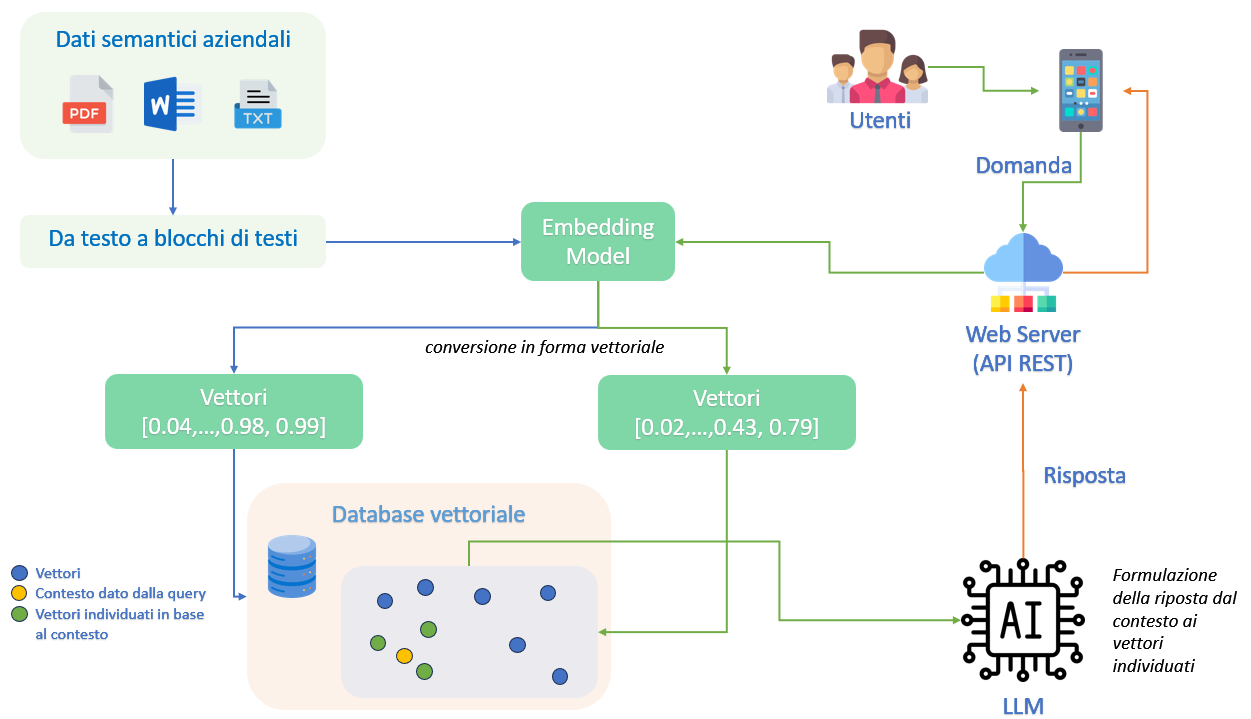
\includegraphics[width=0.8\textwidth]{img/architettura.png}
    \caption{Architettura del prodotto}
    \label{fig:architettura}
\end{figure}

\subsection{Funzionalità del prodotto}
Il prodotto avrà il compito di interagire con i propri utenti attraverso una webapp, rispondendo a domande su cataloghi di bevande. Ogni risposta sarà generata in linguaggio naturale, elaborando i dati tramite \href{https://code7crusaders.github.io/docs/RTB/documentazione_interna/glossario.html#llm-large-language-model}{\textbf{LLM}\textsuperscript{G}}. Le funzionalità principali includono:
\begin{itemize}
    \item \textbf{Interfaccia utente interattiva}: consente agli utenti di porre domande sul catalogo (\textit{es. descrizione di un prodotto o disponibilità in magazzino}) e di ricevere risposte immediate.
    \item \textbf{Motore di ricerca intelligente}: utilizza un sistema di \href{https://code7crusaders.github.io/docs/RTB/documentazione_interna/glossario.html#embedding}{embedding\textsuperscript{G}} per trovare corrispondenze semantiche tra le domande degli utenti e i dati aziendali, estrae il contesto dai dati aziendali per fornire all'\href{https://code7crusaders.github.io/docs/RTB/documentazione_interna/glossario.html#llm-large-language-model}{LLM\textsuperscript{G}} dati accurati da elaborare.
    \item \textbf{Gestione dei dati}: accesso ai dettagli dei prodotti memorizzati in database relazionali, garantendo aggiornamenti in tempo reale. Costruzione di un \href{https://code7crusaders.github.io/docs/RTB/documentazione_interna/glossario.html#database-vettoriale}{database vettoriale\textsuperscript{G}} per l'\href{https://code7crusaders.github.io/docs/RTB/documentazione_interna/glossario.html#embedding}{embedding\textsuperscript{G}} delle parole.
    \item \textbf{Personalizzazione tramite backend}: gli amministratori possono configurare risposte predefinite(\href{https://code7crusaders.github.io/docs/RTB/documentazione_interna/glossario.html#template}{template\textsuperscript{G}} di domanda e risposta), monitorare l’utilizzo e migliorare il sistema tramite feedback utente.
    \item \textbf{Apprendimento continuo}: il sistema evolve grazie ai feedback raccolti dagli utenti, migliorando la qualità delle risposte.
    \item \textbf{Compatibilità multi-dispositivo}: la piattaforma è progettata per essere accessibile 24/7 da mobile e desktop.
\end{itemize}

Il prodotto garantirà inoltre \href{https://code7crusaders.github.io/docs/RTB/documentazione_interna/glossario.html#scalabilità}{scalabilità\textsuperscript{G}} e flessibilità, adattandosi a un’ampia gamma di aziende che desiderano offrire ai propri clienti un’esperienza di interazione avanzata e intuitiva.


\subsection{Tecnologie utilizzate}
Le tecnologie selezionate per la realizzazione del prodotto software sono le seguenti:

\begin{itemize}

    \item \textbf{Embedding Model}: \href{https://code7crusaders.github.io/docs/RTB/documentazione_interna/glossario.html#bert-bidirectional-encoder-representations-from-transformers}{BERT\textsuperscript{G}}\href{https://code7crusaders.github.io/docs/RTB/documentazione_interna/glossario.html#embedding}{\textbf{Embedding\textsuperscript{G}} Model}: BERT (Huggingface) oppure modelli di embedding di Openai (es. Embedding-large) per la trasformazione del testo in vettori semantici. Questo modello viene utilizzato per generare \href{https://code7crusaders.github.io/docs/RTB/documentazione_interna/glossario.html#embedding}{embedding\textsuperscript{G}} efficaci nella fase RAG (Retrieval-Augmented Generation).
    \item \href{https://code7crusaders.github.io/docs/RTB/documentazione_interna/glossario.html#database-relazionale}{\textbf{Database Relazionale}\textsuperscript{G}}: \href{https://code7crusaders.github.io/docs/RTB/documentazione_interna/glossario.html#postgresql}{\textit{PostgreSQL}\textsuperscript{G}} per memorizzare i dati strutturati come cataloghi di prodotti, descrizioni e metadati.
    \item \href{https://code7crusaders.github.io/docs/RTB/documentazione_interna/glossario.html#database-vettoriale}{\textbf{Database Vettoriale}\textsuperscript{G}}: \href{https://code7crusaders.github.io/docs/RTB/documentazione_interna/glossario.html#faiss}{\textit{FAISS}\textsuperscript{G}} per l'archiviazione e il recupero veloce degli embedding e permette un'indicizzazione ottimizzata per la \href{https://code7crusaders.github.io/docs/RTB/documentazione_interna/glossario.html#nearest-neighbor-search-nns}{\textit{nearest neighbor search}\textsuperscript{G}}.
    \item \href{https://code7crusaders.github.io/docs/RTB/documentazione_interna/glossario.html#llm-large-language-model}{\textbf{LLM}\textsuperscript{G}}: OpenAI GPT-4, integrato tramite API OpenAI, per garantire prestazioni elevate e costi scalabili.

\end{itemize}
\begin{figure}[H]

    \centering
    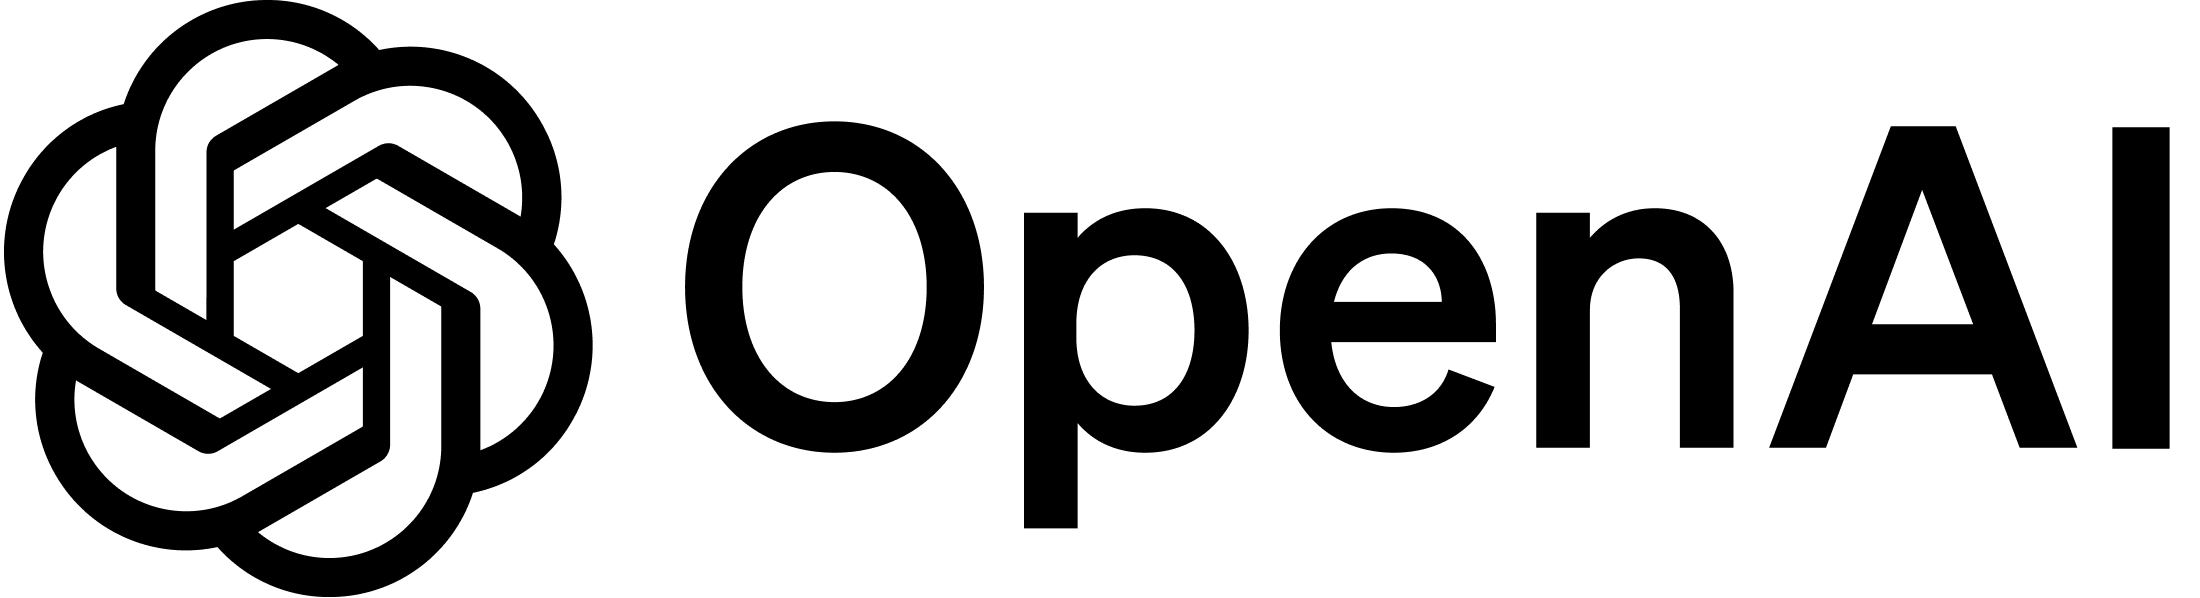
\includegraphics[width=0.2\textwidth]{img/openai-lockup.png}
    \caption{Logo di OpenAI}
    \label{fig:openai_logo}

\end{figure}

\begin{itemize}
    \item \textbf{Web App}: \textit{React} per lo sviluppo dell’interfaccia utente, combinata con \href{https://code7crusaders.github.io/docs/RTB/documentazione_interna/glossario.html#api-rest-representational-state-transfer}{API REST\textsuperscript{G}} per una comunicazione efficiente con il \href{https://code7crusaders.github.io/docs/RTB/documentazione_interna/glossario.html#backend}{backend\textsuperscript{G}}.
    \item \href{https://code7crusaders.github.io/docs/RTB/documentazione_interna/glossario.html#langchain}{\textbf{LangChain}\textsuperscript{G}}: Libreria di orchestrazione utilizzata per integrare \href{https://code7crusaders.github.io/docs/RTB/documentazione_interna/glossario.html#llm-large-language-model}{LLM\textsuperscript{G}}, database vettoriali e pipeline di retrieval.
\end{itemize}

\begin{figure}[H]
    \centering
    
\includegraphics[width=0.2\textwidth]{img/lang-chain.png}
    \caption{Logo di LangChain}
    \label{fig:langchain_logo}
\end{figure}


\subsection{Utenti finali}
Il prodotto è rivolto a aziende che desiderano offrire un servizio di assistenza 
clienti automatizzato e personalizzato. Gli utenti finali sono quindi i clienti 
delle aziende che interagiranno con l’assistente virtuale per ottenere 
informazioni sui prodotti e ricevere supporto.